\chapter{Data Acquisition, Relational Data, and Provenance}
\label{chap:acquisition}
\chapterguide
  {You should understand rows, columns, keys, joins, data quality, and reproducible transformations.}
  {reason about where data come from, identify the grain of a dataset, read relational schemas, write core SQL queries conceptually, recognise collection bias, and document data lineage.}

\section{Analysis starts before the file appears}
A CSV file can make data look self-contained, but every table is the end of a collection process. Someone decided what to measure, when to measure it, which cases to include, how to encode events, and when to stop collecting. Those choices define the evidence available to the analyst.

A useful acquisition record answers at least six questions:
\begin{enumerate}
  \item \textbf{Source:} Which system, organisation, instrument, or study produced the records?
  \item \textbf{Unit:} What does one row represent at the moment of collection?
  \item \textbf{Coverage:} Which people, objects, places, or time periods could appear?
  \item \textbf{Mechanism:} What event causes a record to be created?
  \item \textbf{Version:} Which snapshot or extraction date is being analysed?
  \item \textbf{Transformation:} Which steps occurred between the source and the analytical table?
\end{enumerate}

\begin{keyidea}
Data provenance is part of the dataset. A value without information about how it was produced can be numerically precise but scientifically ambiguous.
\end{keyidea}

\begin{utpfig}[From source systems to an analytical table]{A data-science table is usually produced by several systems and transformations. Each arrow is a place where information can be filtered, duplicated, recoded, delayed, or lost.}{fig:source-to-analysis}
\begin{tikzpicture}[x=1cm,y=1cm]
\node[fcbox,text width=2.2cm] (ops) at (-4.7,1.1) {operational\\database};
\node[fcbox,text width=2.2cm] (sensor) at (-4.7,0) {sensor /\\instrument};
\node[fcbox,text width=2.2cm] (survey) at (-4.7,-1.1) {survey /\\manual entry};
\node[fcbox,text width=2.7cm] (extract) at (-1.5,0) {extract, validate,\\standardise};
\node[fcbox,text width=2.7cm] (store) at (1.8,0) {versioned\\data store};
\node[fcbox,text width=2.8cm] (analysis) at (5.0,0) {analysis-ready\\table};
\draw[fcedge] (ops)--(extract); \draw[fcedge] (sensor)--(extract); \draw[fcedge] (survey)--(extract);
\draw[fcedge] (extract)--(store); \draw[fcedge] (store)--(analysis);
\end{tikzpicture}
\end{utpfig}

\section{Structured, semi-structured, and unstructured data}
\term{Structured data} follow an explicit table-like schema: columns have defined meanings and records repeat a regular structure. Relational databases are the classic example. \term{Semi-structured data} use tags or key--value structure but may allow fields to vary across records; JSON and many event logs fall into this category. \term{Unstructured data} such as free text, images, audio, and video do not naturally arrive as a rectangular feature matrix.

The distinction matters because the analytical work differs. A relational table may require joins and type checks; event logs may require parsing and session construction; text may require tokenisation or embeddings; images require numerical representation before most statistical models can use them.

\begin{dstable}
\begin{tabularx}{\linewidth}{@{}p{3.0cm}p{3.3cm}X@{}}
\toprule
\rowcolor{DSPaleBlue!92}
Data form & Typical example & Questions before analysis \\
\midrule
Structured & transactions table & What is the primary key? What is the row grain? \\
Semi-structured & JSON event log & Which fields are optional? Can schemas change over time? \\
Unstructured & documents or images & How will raw content become measurable features? \\
Time series / streams & sensor readings & Are timestamps reliable? Is ordering preserved? \\
\bottomrule
\end{tabularx}
\end{dstable}

\section{The grain of a table is a scientific decision}
The \term{grain} states exactly what one row represents. A customer table may have one row per customer; a transaction table may have many rows per customer; a sensor table may contain one row per device per minute. Mixing grains without noticing creates duplicated counts, invalid averages, and leakage.

Suppose a hospital dataset contains one row per visit but the question concerns patients. Treating visits as independent people over-represents patients with many visits. Conversely, aggregating visits to one row per patient can remove clinically relevant timing. The correct grain follows from the question.

\begin{utpfig}[Event grain preserves information]{Individual events retain local changes and sequence. Aggregating too early can hide short-lived behaviour and makes some questions impossible to answer later.}{fig:event-grain}
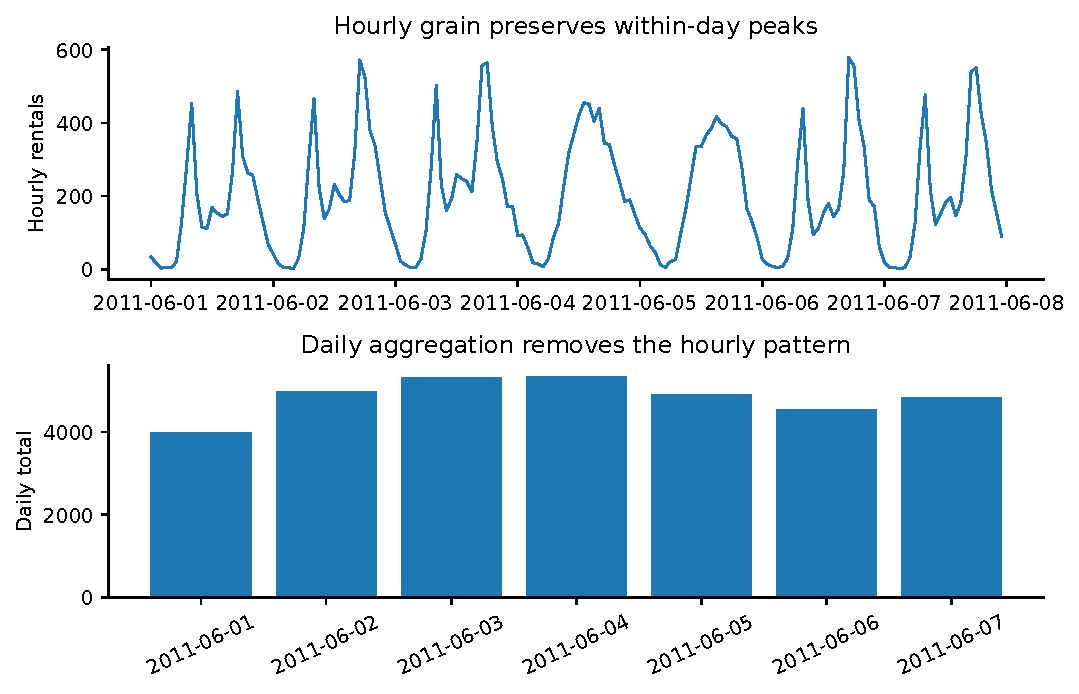
\includegraphics[width=0.86\linewidth]{figures_generated/acq_event_grain.pdf}
\end{utpfig}

\begin{workedexample}
Imagine a retail table with one row per purchase. The mean purchase amount answers a transaction-level question. If the business asks about mean customer spending, first aggregate purchases by customer and then average customer totals. The two quantities are different because frequent customers contribute many transaction rows.
\end{workedexample}

\section{Primary keys, foreign keys, and relational structure}
A \term{primary key} uniquely identifies a row in its table. A \term{foreign key} points from one table to a key in another. These concepts let databases store entities once and connect them without repeating every attribute in every record.

\begin{utpfig}[A small relational schema]{The transaction table records events; customer and product tables record entity attributes. Foreign keys connect the event to the corresponding entities.}{fig:relational-schema}
\begin{tikzpicture}[x=\linewidth,y=1cm,
  schema/.style={draw=UTPBlue!70,fill=UTPPaleBlue,rounded corners=1.5mm,
    line width=0.6pt,text width=0.26\linewidth,minimum height=2.55cm,
    inner xsep=2.5mm,inner ysep=2mm,align=left,
    font=\scriptsize\color{UTPNavy}},
  flow/.style={-{Stealth[length=2mm,width=1.5mm]},
    line width=0.8pt,draw=UTPTeal,rounded corners=1.5mm}]
\node[schema] (cust) at (0,1.5) {\textbf{customers}\\[5pt]
  \texttt{customer\_id} \textbf{(PK)}\\
  \texttt{region}\\
  \texttt{join\_date}};
\node[schema] (prod) at (0,-1.5) {\textbf{products}\\[5pt]
  \texttt{product\_id} \textbf{(PK)}\\
  \texttt{category}\\
  \texttt{unit\_price}};
\node[schema] (tx) at (0.335,0) {\textbf{transactions}\\[5pt]
  \texttt{transaction\_id} \textbf{(PK)}\\
  \texttt{customer\_id} \textbf{(FK)}\\
  \texttt{product\_id} \textbf{(FK)}\\
  \texttt{timestamp}\\
  \texttt{quantity}};
\node[schema,draw=UTPTeal!80,fill=UTPPaleTeal,align=center] (fact) at (0.670,0)
  {\textbf{Analysis table}\\[5pt]
   One row\\per transaction};
\draw[flow] (cust.east) -- (0.1675,1.5) -- (0.1675,0.4) --
  ([yshift=4mm]tx.west);
\draw[flow] (prod.east) -- (0.1675,-1.5) -- (0.1675,-0.4) --
  ([yshift=-4mm]tx.west);
\draw[flow] (tx.east) -- (fact.west);
\node[font=\scriptsize\color{UTPMuted},align=center,
  text width=0.85\linewidth] at (0.335,-3.15)
  {\textbf{PK}: primary key \qquad \textbf{FK}: foreign key};
\end{tikzpicture}
\end{utpfig}

Relational design also forces analysts to ask whether keys are truly unique. A supposed customer identifier that appears with conflicting birth dates is not just a database inconvenience: it signals an identity-resolution or data-quality problem.

\section{Join cardinality predicts what a join can do}
Before joining, describe the relationship between keys:
\begin{itemize}
  \item \textbf{one-to-one}: each key occurs once in both tables;
  \item \textbf{one-to-many}: one entity row connects to many event rows;
  \item \textbf{many-to-many}: both tables repeat the join key.
\end{itemize}
Many-to-many joins can multiply rows dramatically. This may be correct, but it must be intentional.

\begin{utpfig}[Cardinality determines row multiplication]{A one-to-many relationship is expected when one customer has several transactions. A many-to-many relationship creates every compatible pair and can inflate counts if the analyst expected a one-to-one merge.}{fig:join-cardinality-acq}
\begin{tikzpicture}[x=\linewidth,y=1cm,
  rowbox/.style={draw=UTPBlue!70,fill=UTPPaleBlue,rounded corners=1mm,
    line width=0.6pt,text width=0.085\linewidth,minimum height=0.60cm,
    inner xsep=1mm,inner ysep=1mm,align=center,
    font=\scriptsize\color{UTPNavy}},
  matched/.style={rowbox,draw=UTPTeal!80,fill=UTPPaleTeal},
  repeated/.style={rowbox,draw=UTPRed!80,fill=UTPPaleRed},
  matchflow/.style={-{Stealth[length=1.7mm,width=1.3mm]},
    line width=0.6pt,draw=UTPTeal},
  heading/.style={font=\scriptsize\bfseries\color{UTPNavy},align=center},
  tablelabel/.style={font=\scriptsize\color{UTPMuted},align=center}]
\node[heading] at (0.215,1.9) {One-to-many};
\node[heading] at (0.745,1.9) {Many-to-many};
\foreach \x in {0.09,0.62}{
  \node[tablelabel] at (\x,1.3) {Left table};
}
\foreach \x in {0.34,0.87}{
  \node[tablelabel] at (\x,1.3) {Right table};
}
\node[rowbox] (a1) at (0.09,0) {key = A};
\node[matched] (b1) at (0.34,0.8) {key = A};
\node[matched] (b2) at (0.34,0) {key = A};
\node[matched] (b3) at (0.34,-0.8) {key = A};
\foreach \b in {b1,b2,b3}{\draw[matchflow] (a1.east) -- (\b.west);}
\node[repeated] (c1) at (0.62,0.4) {key = A};
\node[repeated] (c2) at (0.62,-0.4) {key = A};
\node[repeated] (d1) at (0.87,0.8) {key = A};
\node[repeated] (d2) at (0.87,0) {key = A};
\node[repeated] (d3) at (0.87,-0.8) {key = A};
\foreach \c in {c1,c2}{
  \foreach \d in {d1,d2,d3}{
    \draw[matchflow,draw=UTPRed!80] (\c.east) -- (\d.west);
  }
}
\draw[UTPMuted!35,line width=0.5pt] (0.48,1.9) -- (0.48,-1.65);
\node[heading,text=UTPTeal!85!black] at (0.215,-1.45)
  {$1 \times 3 = 3$ joined rows};
\node[heading,text=UTPRed!85!black] at (0.745,-1.45)
  {$2 \times 3 = 6$ joined rows};
\node[tablelabel] at (0.48,-2.05)
  {Each arrow represents one matching pair in the join.};
\end{tikzpicture}
\end{utpfig}

\section{SQL expresses data transformations close to the source}
Structured Query Language (SQL) is widely used to select, filter, aggregate, and join relational data before it reaches R or another analysis environment. The exact database dialect varies, but the core logic is stable.

\begin{lstlisting}[style=dsr]
-- Conceptual SQL: one row per region
SELECT
    c.region,
    COUNT(*) AS transactions,
    SUM(t.quantity * p.unit_price) AS revenue
FROM transactions AS t
JOIN customers AS c
  ON t.customer_id = c.customer_id
JOIN products AS p
  ON t.product_id = p.product_id
WHERE t.timestamp >= '2026-01-01'
GROUP BY c.region;
\end{lstlisting}

Read the query from the analytical grain outward. The joins first construct transaction records enriched with customer and product attributes. The filter defines the time window. The grouping then changes the grain from transactions to regions.

\begin{pitfall}
A database can execute a syntactically valid query that answers the wrong question. SQL correctness does not replace reasoning about grain, keys, filters, and denominators.
\end{pitfall}

\section{Collection mechanisms create selection effects}
A dataset is rarely a simple random sample of everything the analyst cares about. Records may exist only for users who interact with a product, patients who reach a clinic, sensors that remain online, or survey respondents who choose to participate.

\begin{utpfig}[Collection bias changes composition]{The available dataset can over-represent some groups and under-represent others even when every recorded row is internally correct.}{fig:acq-sampling-bias}
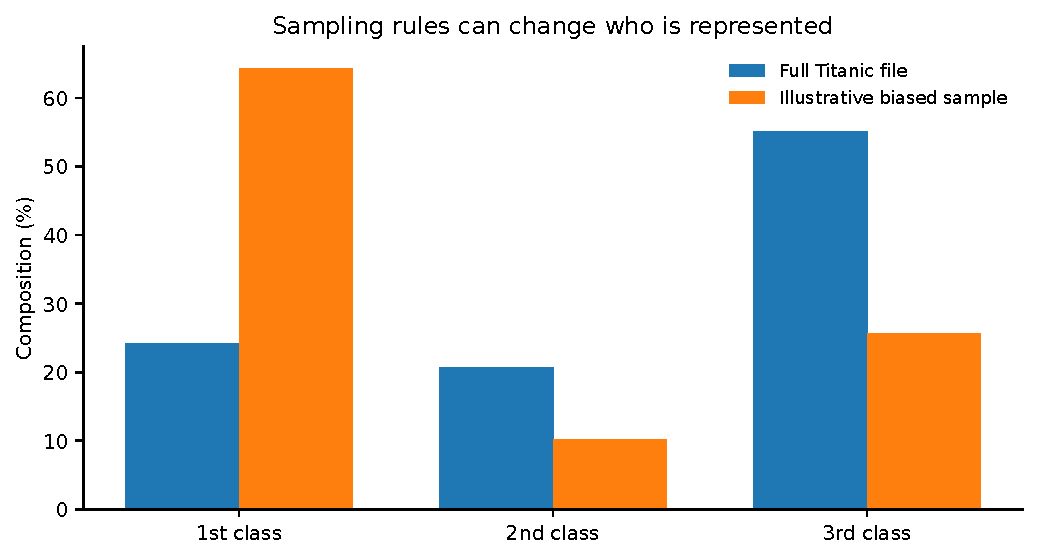
\includegraphics[width=0.82\linewidth]{figures_generated/acq_sampling_bias.pdf}
\end{utpfig}

This distinction separates \term{data quality within the sample} from \term{representativeness of the sample}. Cleaning cannot repair a population that was never observed.

\section{Time creates ordering, delay, and censoring problems}
Time-stamped data require more than parsing a date column. Ask whether the timestamp represents occurrence time, recording time, update time, or extraction time. A transaction may occur at 11:58 p.m. but reach a reporting system after midnight; a medical outcome may only be known weeks later.

Important temporal concepts include:
\begin{itemize}
  \item \textbf{latency}: delay between an event and its availability;
  \item \textbf{censoring}: the observation window ends before an outcome is fully known;
  \item \textbf{seasonality}: predictable calendar-related patterns;
  \item \textbf{concept drift}: the relationship between features and target changes over time;
  \item \textbf{look-ahead leakage}: future information enters a model meant to predict the past.
\end{itemize}

\begin{utpfig}[Occurrence time is not always availability time]{For predictive work, a feature is valid only if it would have been available at the actual decision time.}{fig:availability-timeline}
\begin{tikzpicture}[x=1cm,y=1cm]
\draw[-{Stealth[length=2mm]},thick,draw=UTPMuted] (-5,0)--(5,0);
\foreach \x/\lab in {-4/{event},-1.2/{decision},1.4/{outcome},3.8/{record updated}}{
  \draw[thick,draw=UTPBlue] (\x,-.16)--(\x,.16); \node[tagb,align=center] at (\x,-.55) {\lab};
}
\draw[very thick,draw=UTPGreen] (-4,.45)--(-1.2,.45);
\node[tag,align=center] at (-2.6,.78) {information genuinely available};
\draw[very thick,draw=UTPRed] (1.4,.45)--(3.8,.45);
\node[tag,align=center,text=UTPRed] at (2.6,.78) {future information: leakage if used};
\end{tikzpicture}
\end{utpfig}

\section{Data lineage turns transformations into an inspectable chain}
\term{Lineage} records how an output was produced from upstream inputs. At minimum, preserve source filenames or table versions, extraction dates, code versions, transformation scripts, and generated outputs.

\begin{utpfig}[Lineage as a directed graph]{If an analysis result changes, lineage makes it possible to trace the change back through model code, features, cleaning rules, and source data.}{fig:data-lineage}
\begin{tikzpicture}[x=\linewidth,y=1cm,
  artifact/.style={draw=UTPBlue!70,fill=UTPPaleBlue,rounded corners=1.5mm,
    line width=0.6pt,text width=0.14\linewidth,minimum height=1.45cm,
    inner xsep=1.8mm,inner ysep=2mm,align=center,
    font=\scriptsize\color{UTPNavy}},
  connector/.style={line width=0.8pt,draw=UTPTeal,rounded corners=1.5mm},
  flow/.style={connector,-{Stealth[length=1.8mm,width=1.4mm]}}]
\node[artifact] (raw) at (0,0) {\textbf{Raw snapshot}\\[4pt]
  Versioned\\source data};
\node[artifact] (clean) at (0.20,0) {\textbf{Clean table}\\[4pt]
  Checked\\records};
\node[artifact] (feat) at (0.40,0) {\textbf{Feature table}\\[4pt]
  Derived\\variables};
\node[artifact] (model) at (0.60,1.05) {\textbf{Model}\\[4pt]
  Fitted\\model};
\node[artifact] (report) at (0.60,-1.05) {\textbf{Report}\\[4pt]
  Evidence and\\interpretation};
\node[artifact,draw=UTPTeal!80,fill=UTPPaleTeal] (decision) at (0.80,0)
  {\textbf{Handoff}\\[4pt]
   Decision and\\delivery};
\coordinate (split) at (0.50,0);
\coordinate (merge) at (0.70,0);
\draw[flow] (raw.east) -- (clean.west);
\draw[flow] (clean.east) -- (feat.west);
\draw[connector] (feat.east) -- (split);
\draw[flow] (split) |- (model.west);
\draw[flow] (split) |- (report.west);
\draw[connector] (model.east) -| (merge);
\draw[connector] (report.east) -| (merge);
\draw[flow] (merge) -- (decision.west);
\end{tikzpicture}
\end{utpfig}

\section{Version data when meaning can change}
A filename such as \texttt{final.csv} does not identify a stable dataset. Useful versioning records either immutable snapshots or a reproducible recipe for reconstructing them. Schema changes should be treated as versioned changes as well: renaming a category, changing a unit, or redefining a target can alter results even when row counts remain similar.

\begin{referencebox}
A practical project can keep a small manifest containing: dataset name, source page, extraction or download date, row count, column count, checksum, schema notes, and the script that produced the analytical version. This is especially useful when external files may later change.
\end{referencebox}

\section{Batch and streaming systems answer different operational needs}
\term{Batch processing} collects data over a period and processes it together. \term{Streaming processing} handles events continuously or in short windows. The statistical ideas are similar, but operations differ: streams require handling late events, duplicated messages, changing schemas, and continuous monitoring.

\begin{utpfig}[Batch versus stream]{Batch pipelines emphasise repeatable snapshots. Streaming pipelines emphasise event ordering, latency, and continuous quality checks.}{fig:batch-stream}
\begin{tikzpicture}[x=\linewidth,y=1cm,
  stage/.style={draw=UTPBlue!70,fill=UTPPaleBlue,rounded corners=1.5mm,
    line width=0.6pt,text width=0.19\linewidth,minimum height=1.45cm,
    inner xsep=2mm,inner ysep=2mm,align=center,
    font=\scriptsize\color{UTPNavy}},
  output/.style={stage,draw=UTPTeal!80,fill=UTPPaleTeal},
  flow/.style={-{Stealth[length=2mm,width=1.5mm]},
    line width=0.8pt,draw=UTPTeal},
  heading/.style={font=\scriptsize\bfseries\color{UTPNavy},anchor=west}]
\node[heading] at (-0.107,1.1)
  {Batch: process a collected period together};
\node[stage] (b1) at (0,0) {\textbf{Collected events}\\[4pt]
  A day of\\records};
\node[stage] (b2) at (0.25,0) {\textbf{Scheduled job}\\[4pt]
  Nightly\\processing};
\node[output] (b3) at (0.50,0) {\textbf{Daily table}\\[4pt]
  Repeatable\\snapshot};
\draw[flow] (b1.east) -- (b2.west);
\draw[flow] (b2.east) -- (b3.west);
\draw[UTPMuted!35,line width=0.5pt] (-0.107,-1.05) -- (0.857,-1.05);
\node[heading] at (-0.107,-1.5)
  {Stream: process events as they arrive};
\node[stage] (s1) at (0,-2.65) {\textbf{Event}\\[4pt]
  New incoming\\record};
\node[stage] (s2) at (0.25,-2.65) {\textbf{Validate / transform}\\[4pt]
  Check and\\prepare data};
\node[stage] (s3) at (0.50,-2.65) {\textbf{Live state}\\[4pt]
  Continuously\\updated};
\node[output] (s4) at (0.75,-2.65) {\textbf{Monitor}\\[4pt]
  Latency and\\data quality};
\draw[flow] (s1.east) -- (s2.west);
\draw[flow] (s2.east) -- (s3.west);
\draw[flow] (s3.east) -- (s4.west);
\end{tikzpicture}
\end{utpfig}

\section{A practical acquisition checklist}
Before analysing externally supplied data, record the following:
\begin{enumerate}
  \item State the source and intended population.
  \item Define one row precisely.
  \item Identify candidate primary keys and verify uniqueness where expected.
  \item Record extraction dates and time coverage.
  \item Compare the collected sample with any known reference population.
  \item Preserve raw data separately from cleaned or derived data.
  \item Document every join and expected cardinality.
  \item Record exclusions and filters with reasons.
  \item Keep provenance sufficient to reconstruct the analytical table.
\end{enumerate}

\begin{quickcheck}
\begin{enumerate}
  \item Why can a perfectly clean sample still be unrepresentative?
  \item What is the difference between a primary key and a foreign key?
  \item Why should join cardinality be checked before a join?
  \item What is look-ahead leakage in time-dependent data?
  \item Which provenance information would you need to reproduce a table six months later?
\end{enumerate}
\end{quickcheck}

\section{Worked provenance example: the same system at two grains}

The bundled Bike Sharing data arrive as both daily and hourly tables. They describe the same rental system, but they are not interchangeable datasets.

\begin{utpfig}[Daily and hourly data have different grains]{The daily file contains 731 rows while the hourly file contains 17,379 rows. More rows do not automatically mean more independent information; many hourly observations share the same calendar day, season, and broader weather context.}{fig:acq-bike-grain}
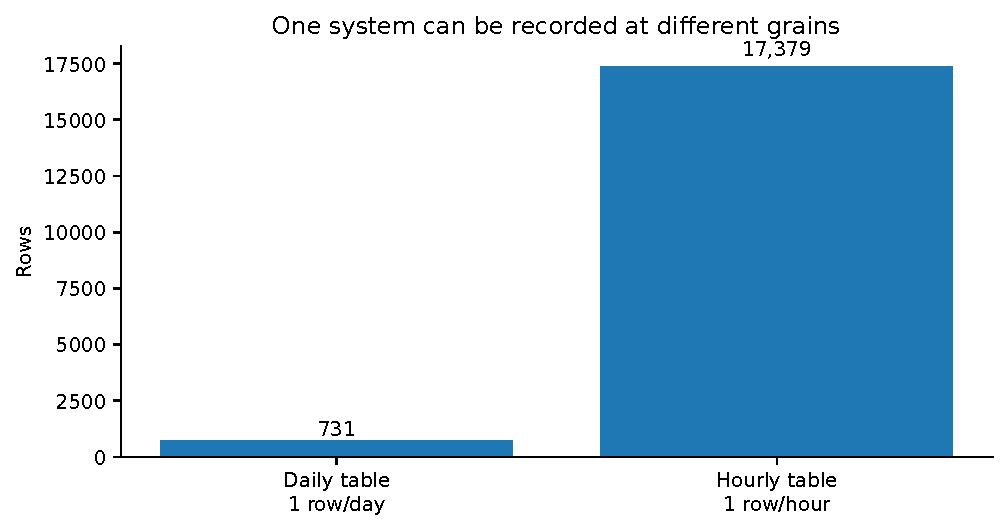
\includegraphics[width=0.72\linewidth]{figures_generated/acq_bike_grain_comparison.pdf}
\end{utpfig}

If the question concerns commuter peaks, the daily table has already aggregated away the relevant within-day variation. If the question concerns long seasonal change, the hourly table may be unnecessarily granular and repeated observations within a day must be handled carefully. A provenance record should therefore capture not just the filename and source but the \textbf{unit of observation, time coverage, aggregation rule, and known transformations}.

\begin{keyidea}
Grain is part of provenance. Two files can contain the same variable names and still support different claims because one row means something different.
\end{keyidea}

\begin{chapterrecap}
\begin{itemize}
  \item Data acquisition determines what the analysis can legitimately represent.
  \item Grain, keys, and time semantics should be explicit before transformation.
  \item SQL is a language for expressing relational transformations, not a substitute for analytical reasoning.
  \item Collection mechanisms can create selection bias even when recorded values are accurate.
  \item Provenance and lineage make analytical results traceable and reproducible.
\end{itemize}
\end{chapterrecap}
